\documentclass[11pt]{article}

\usepackage[margin=0.75in]{geometry}
\usepackage[T1]{fontenc}
\usepackage{amsmath,amssymb}
\usepackage{booktabs}
\usepackage{graphicx}
\usepackage{tabularx}
\usepackage{threeparttable}

\newcolumntype{Y}{>{\raggedright\arraybackslash}X}
\newcolumntype{Z}{>{\centering\arraybackslash}X}

\title{Supplementary Appendix}
\author{}
\date{}

\begin{document}

\maketitle

\section*{Supplementary Appendix A. Graph-learning and target-extraction notation}

\begin{table}[p]
\centering
\caption{GNN notation.}
\begin{threeparttable}
\scriptsize
\setlength{\tabcolsep}{3pt}
\renewcommand{\arraystretch}{0.97}
\begin{tabularx}{\textwidth}{Z Z Y}
\toprule
Symbol & Type & Definition \\
\midrule
$I$ & Set & Zones (graph nodes). \\
$E$ & Set & Graph edges between zones. \\
$T$ & Set & Time steps used for learning. \\
$P$ & Parameter & Number of time-varying mobility features. \\
$R$ & Parameter & Number of static zone attributes. \\
$L$ & Parameter & Number of spatial message-passing layers. \\
$\mathcal{G}$ & Object & Weighted urban graph $(I,E,\mathbf{W})$. \\
$\mathcal{N}(i)$ & Set & Neighbor set of zone $i$. \\
$w_{ij}$ & Parameter & Edge weight from zone $i$ to zone $j$. \\
$t_{ij}$ & Parameter & Network travel time between zones. \\
$\tau$ & Parameter & Scale parameter in edge-weight decay. \\
$\mathbf{x}_{i,t}$ & Input vector & Node features for zone $i$ at time $t$. \\
$\mathbf{X}_t$ & Input matrix & Stacked node features at time $t$. \\
$\mathbf{W}_s^{(l)},\mathbf{U}_s^{(l)}$ & Parameter & Trainable spatial weight matrices at layer $l$. \\
$\sigma(\cdot)$ & Operator & Nonlinear activation in the spatial propagation step. \\
$\mathbf{h}_{i,t}^{(l)}$ & Latent state & Spatial embedding at layer $l$. \\
$\mathbf{g}_{i,t}$ & Latent state & Temporal embedding after recurrent update. \\
$f_{\mathrm{out}}(\cdot)$ & Operator & Output head mapping latent states to predicted demand. \\
$\hat{y}_{i,t}$ & Output & Predicted charging-demand intensity. \\
$y_{i,t}$ & Target & Observed/proxy demand intensity for training. \\
$T_{\mathrm{train}}$ & Set & Training subset of time steps. \\
$\mathbf{r}_t$ & Latent state & Mean latent representation used in temporal attention. \\
$\mathbf{q},\mathbf{W}_a$ & Parameter & Trainable attention parameters. \\
$\alpha_t$ & Output & Temporal attention weight at time $t$. \\
$s_i^{\mathrm{raw}}$ & Derived output & Raw zone-level priority score from ST-GNN outputs. \\
$s_i$ & Derived output & Normalized priority index used in optimization. \\
$T_v$ & Set & Venue-relevant time window associated with venue type $v$. \\
$\omega_{iv}$ & Derived output & Venue-specific share weight for zone $i$. \\
\bottomrule
\end{tabularx}
\end{threeparttable}
\end{table}

\clearpage

\section*{Supplementary Appendix B. Optimization-and-equity notation}

\begin{table}[p]
\centering
\caption{Optimization and equity notation.}
\begin{threeparttable}
\scriptsize
\setlength{\tabcolsep}{3pt}
\renewcommand{\arraystretch}{0.97}
\begin{tabularx}{\textwidth}{Z Z Y}
\toprule
Symbol & Type & Definition \\
\midrule
$V$ & Set & Venue types (residential, workplace, public). \\
$M$ & Set & Vulnerability indicators. \\
$\mathcal{V}^{Q}$ & Set & Most vulnerable quartile of zones used for quartile-share and coverage reporting. \\
$\mathcal{V}^{H}$ & Set & High-vulnerability zones for floor constraints. \\
$Q_v$ & Parameter & Exogenous quota of ports for venue $v$. \\
$\pi_{iv}$ & Parameter & Share for zone $i$, venue $v$, from the target-allocation equation in the main text. \\
$T_{iv}$ & Parameter & Priority-preserving target ports for zone $i$, venue $v$. \\
$z_{im}$ & Parameter & Standardized vulnerability indicator $m$ in zone $i$. \\
$\eta_m$ & Parameter & Indicator weight in vulnerability index. \\
$\nu_i$ & Parameter & Social charging vulnerability index for zone $i$. \\
$\lambda_v$ & Parameter & Venue-specific decay coefficient in accessibility (minutes). \\
$\varepsilon$ & Parameter & Tolerance for loss of priority fidelity. \\
$U^{\star}$ & Parameter & Optimal upper-level objective value. \\
$\underline{A}$ & Parameter & Accessibility floor for $\mathcal{V}^{H}$. \\
$\kappa$ & Parameter & Intensity parameter for vulnerability weighting in the socially weighted equity objective. \\
$S^{Q}$ & Metric & Share of total accessibility captured by $\mathcal{V}^{Q}$. \\
$C^{15}$ & Metric & Share of zones in $\mathcal{V}^{Q}$ with at least one allocated port reachable within 15 minutes. \\
$G_{\mathrm{W}}$ & Metric & Vulnerability-weighted accessibility Gini computed with zone weights $1+\nu_i$. \\
$\bar{\nu}_{ij}$ & Parameter & Pairwise vulnerability weight used in the socially weighted lower-level objective. \\
$\gamma$ & Parameter & Relaxation factor used to define the soft accessibility floor in S3. \\
$q_{0.10}(\cdot)$ & Operator & Tenth-percentile operator used to calibrate the soft floor. \\
$\beta$ & Parameter & Penalty weight on protected-zone shortfalls in S3. \\
$n_{iv}$ & Decision variable & Integer ports allocated to zone $i$, venue $v$. \\
$u_{iv}$ & Decision variable & Absolute deviation from target $T_{iv}$. \\
$A_i$ & Metric & Accessibility experienced by demand zone $i$. \\
$z_{ij}$ & Decision variable & Linearized absolute accessibility gap between $i$ and $j$. \\
$d_i$ & Decision variable & Nonnegative shortfall variable for the soft floor in protected zones. \\
\bottomrule
\end{tabularx}
\end{threeparttable}
\end{table}

\clearpage

\section*{Supplementary Appendix C. Additional figures}

\begin{figure}[p]
\centering
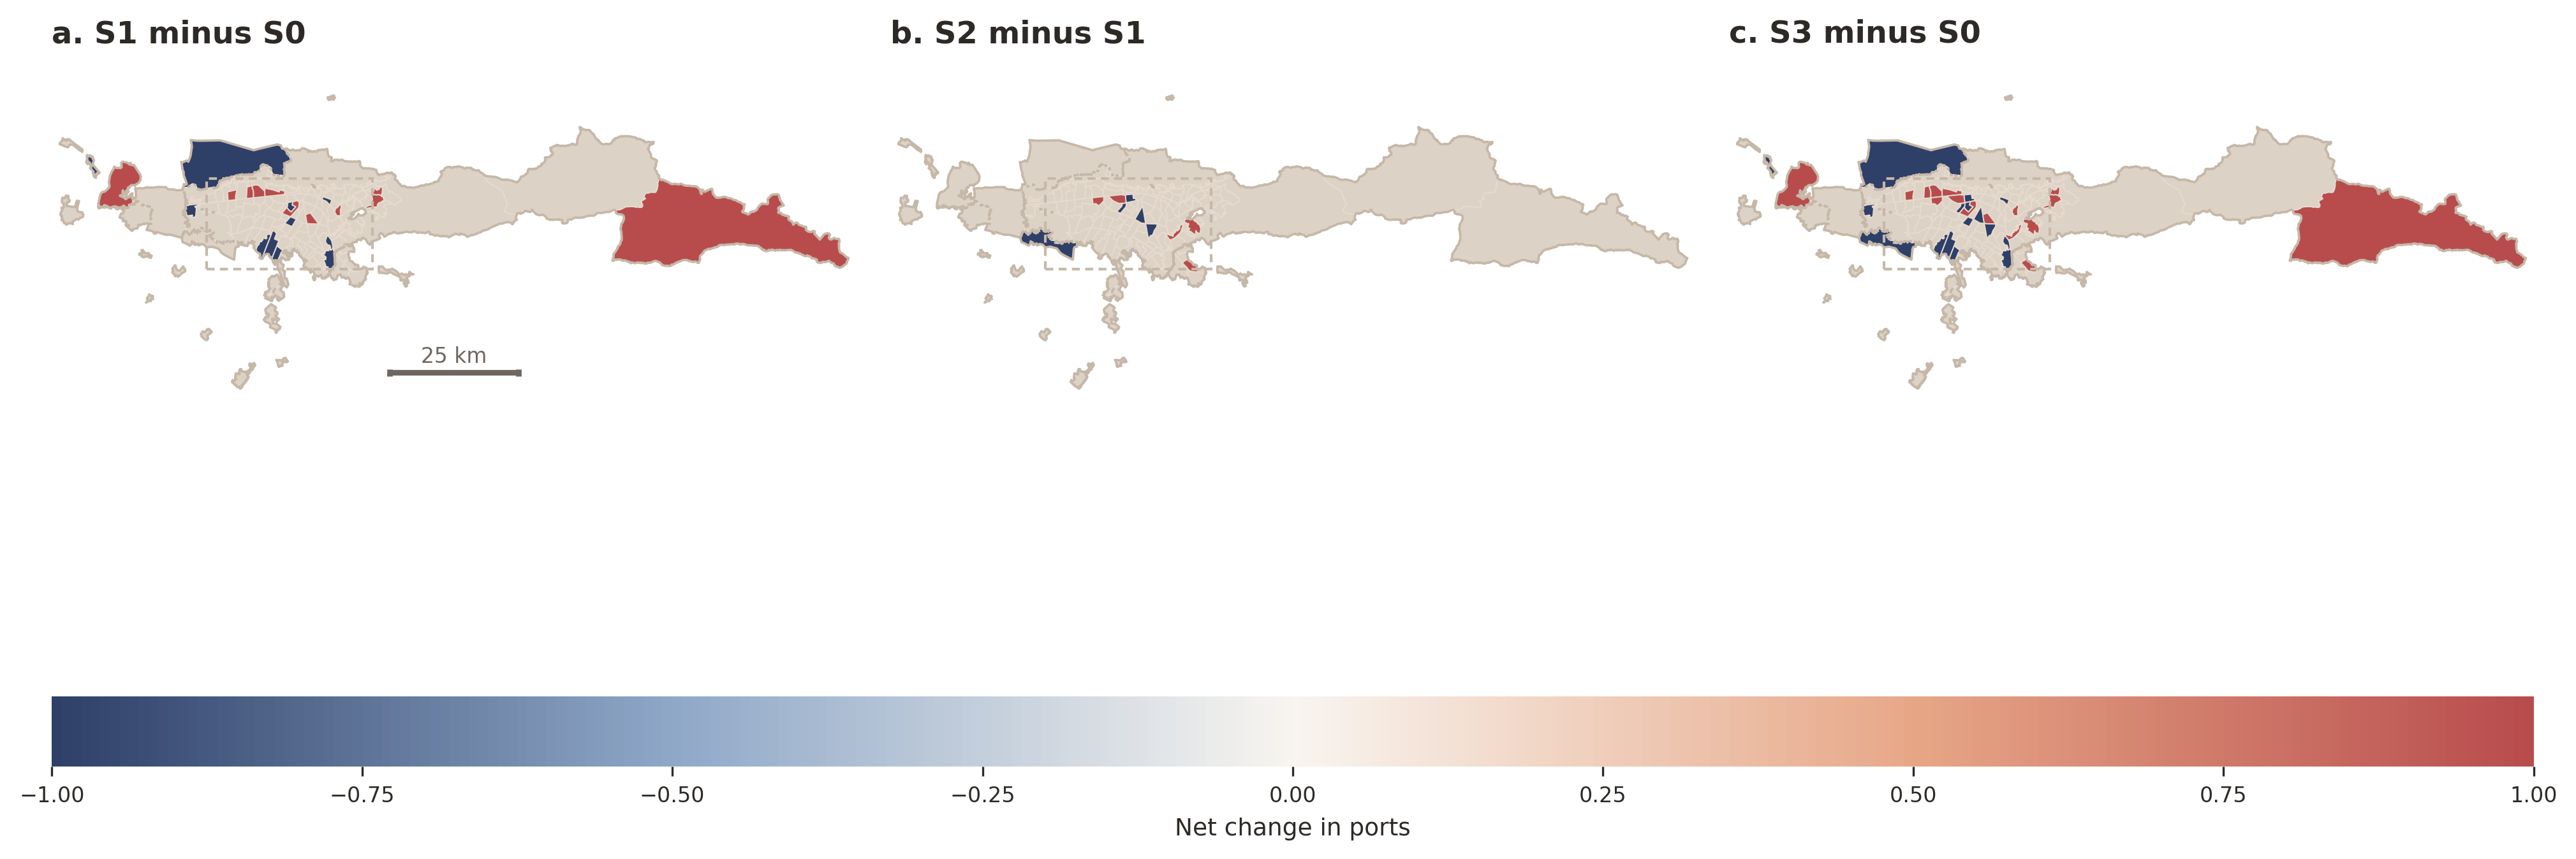
\includegraphics[width=\textwidth]{figures/fig_growth_progression.png}
\caption{Growth-progression maps across allocation stages. The panels expand the stage-to-stage spatial story behind the final allocation comparison and provide supplementary spatial detail on how the scenario sequence evolves under fixed quotas.}
\end{figure}

\begin{figure}[p]
\centering
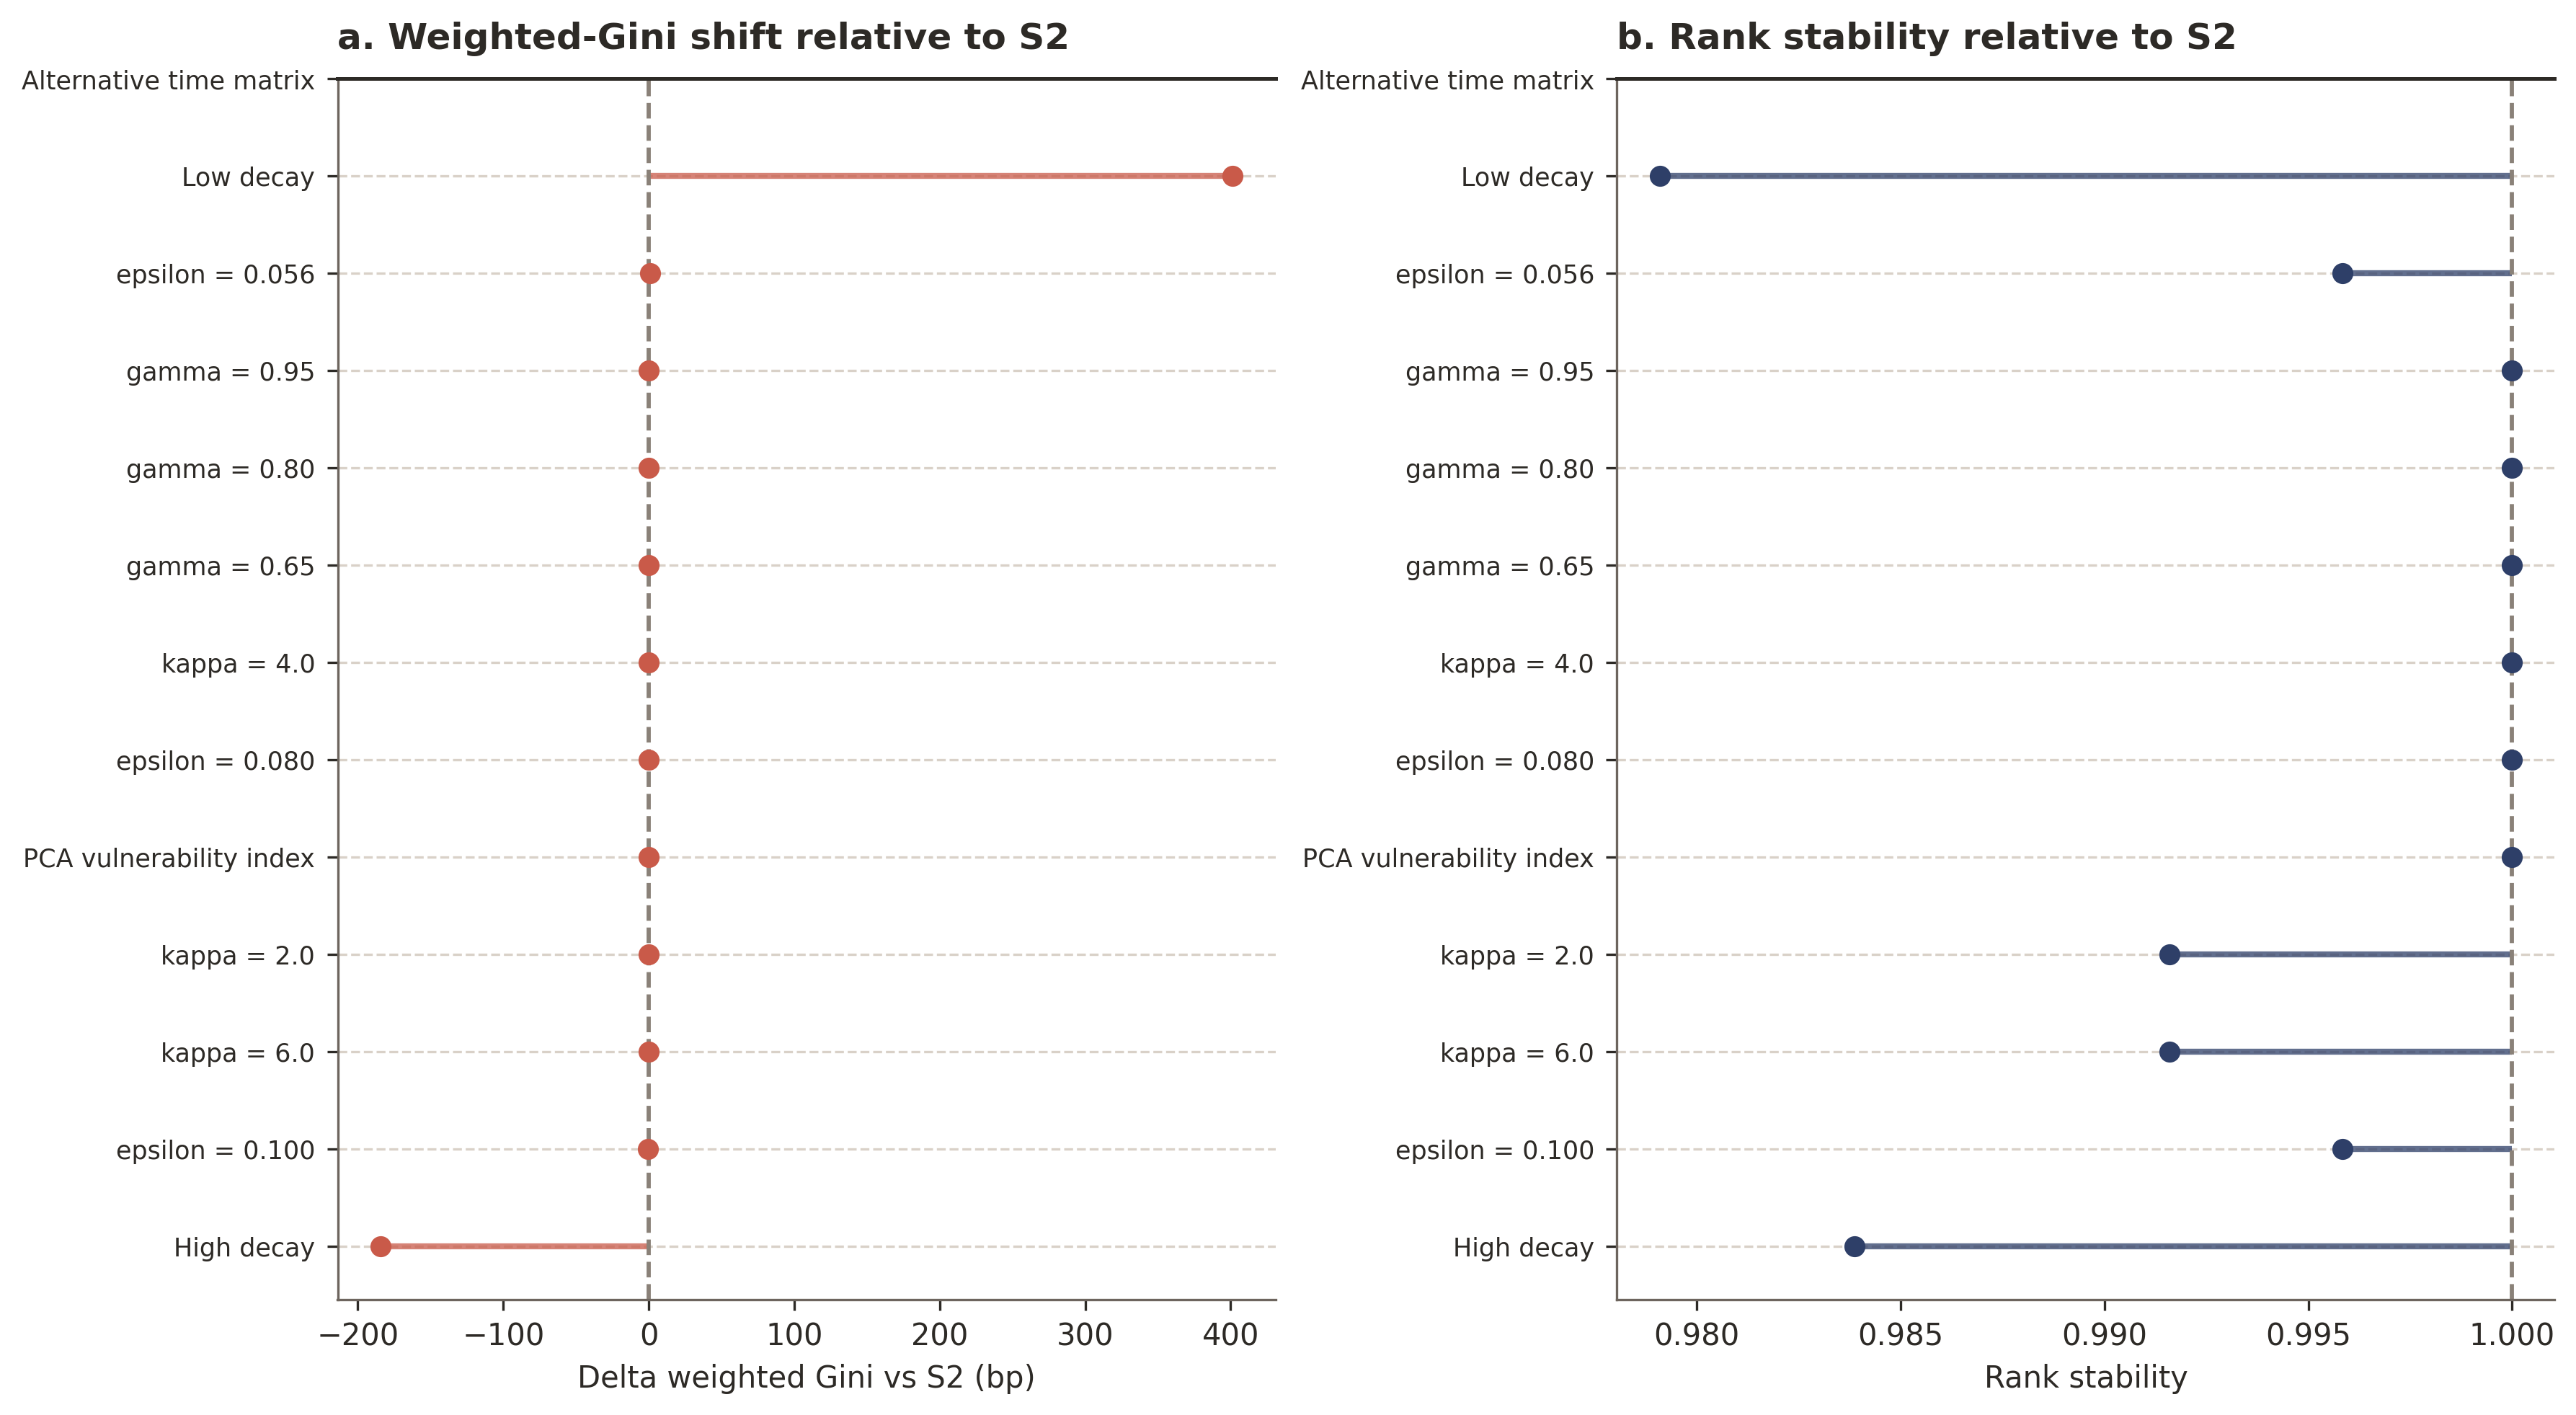
\includegraphics[width=\textwidth]{figures/fig_robustness.png}
\caption{Robustness checks around the S2 baseline. The main scenario ordering and high rank stability are preserved across alternative decay, vulnerability-index, epsilon, kappa, and soft-floor specifications, while the strongest sensitivity appears in the accessibility-decay calibration.}
\end{figure}

\end{document}